\chapter{Annexes}
\label{annexe:gantt}

	\section{Simplification en eaux profondes}

		Nous allons ici justifier la simplification faite en eaux profondes dans la \textsc{Section}~\ref{sec:simplification_eaux_profondes}. Nous avons en effet pu proposer une approximation en \textsc{Equation}~\ref{eqn:simplification_eaux_profondes} qui permet de simplifier les équations décrivant la dynamique du milieu marin.

		\begin{eqnarray}
			\frac{cosh(k_m(z+H))}{sinh(k_mH)} = \left( \frac{e^{z+H} + e^{-z+H}}{e^{H}-e^{-H}} \right)^{k_m}  \xrightarrow[H \rightarrow + \infty]{}   \left( \frac{e^{z+H}}{e^{H}} \right)^{k_m} = e^{k_m z}
		\end{eqnarray}

		Pour la simplification de l'\textsc{Equation}~\ref{equation:dispersion} en l'\textsc{Equation}~\ref{equation:deep_dispersion} de dispersion des vagues, cela se justifie par le fait que :

		\begin{eqnarray}
			tanh(k_m H) \xrightarrow[H \rightarrow + \infty]{} 1
		\end{eqnarray}

	\section{Volume d'une calotte sphérique}

		Nous allons justifier l'\textsc{Equation}~\ref{eqn:v_immerge} qui donne le volume d'une calotte sphérique afin de déterminer le volume immergé d'une sphère. L'idée est d'obtenir le volume par intégration en remarquant que le volume est engendré par la rotation du triangle curviligne O $(0, 0)$ H $(h, 0)$ M $(h, f(h))$, comme le montre la \textsc{Figure}~\ref{fig:calotte_spherique}, on a :

		\begin{figure}[!htb]
			\centering
			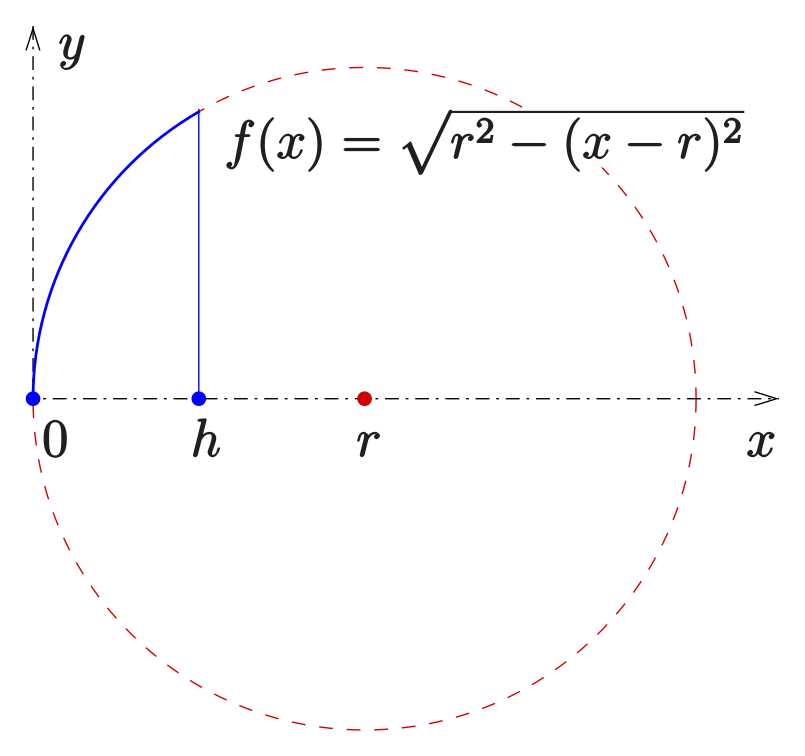
\includegraphics[width=0.4\textwidth]{imgs/calotte_spherique.png}
			\caption{Périmètre d'une calotte sphérique, Ag2gaeh, 2015, \url{https://fr.wikipedia.org/wiki/Calotte_sphérique}}
			\label{fig:calotte_spherique}
		\end{figure}

		\begin{equation}
			V_i = \pi \int_0^h f^2(x).dx = \pi \int_0^h (2rx - x^2).dx = \pi \left[(rx^2 - \frac{x^3}{3})\right]_0^h = \pi h^2 \frac{3r - h}{3}
		\end{equation}

	\clearpage

	\section{Diagrammes de Gantt}

	\begin{figure}[H]
		\centering
		\rotatebox{90}{
			\includegraphics[width=20cm]{gantt_before.pdf}
		}
        \label{fig:gantt_before}
        \caption{Diagramme de Gantt prévisionnel du projet}
	\end{figure}

	\begin{figure}[H]
		\centering
		\rotatebox{90}{
			\includegraphics[width=20cm]{gantt_after.pdf}
		}
        \label{fig:gantt_after}
        \caption{Diagramme de Gantt final du projet}
	\end{figure}